\chapter{Deep Reinforcement Learning in Chess (and other games)}
\label{ch:drlgames}
In this chapter, we will explore how we can use deep \gls{rl} and mechanisms discussed in previous chapters to let a machine play games, and chess especially as it is the main focus of this dissertation. As we will have to feed chess positions into the neural networks, we will have to transform them into a vector representation. One should not forget that the starting point of the machine should be only knowledge about the game, and no expert knowledge. How this is done and how we can do it in chess is discussed in section \ref{sec:fs}. We need a function transforming this vector data into an evaluation, this is considered in \ref{sec:sef}. The application of TD($\lambda$) and more sophisticated versions of TD-learning to games is further examined in section \ref{sec:td}. A method that has shown recent success is presented in section \ref{sec:mcts} and we conclude this chapter by also considering how we could introduce policy iterations into chess in section \ref{sec:polnet}.

\section{Feature Space}
\label{sec:fs}
Because the state space of most games is excessively big, tabular methods have no chance of being successful. This fact justifies using function approximation on a vectorized representation of game states. The feature vector is then fed into a machine learning framework of choice, often (deep) neural networks and \gls{cnn}s.\\

The goal of our feature vector should be general and low level enough, to avoid being biased by the features. Let us examine the chess representations used by other machine learning engines for inspiration.\\
In section \ref{sec:evaluation} we already described how most engines represent the chess position with handcrafted expert features among features that only contain knowledge strictly characteristic to the model of the game. Also \textit{Meep}, a \gls{rl} based chess program, maintains
\begin{itemize}
\item material
\item piece square tables
\item pawn structure
\item mobility
\item king safety
\end{itemize}
information in a mostly binary fashion, which makes it a sparse representation \cite{veness09}. To arrive to a unbiased and general representation of the chess board, we will combine ideas from computer vision and another board game, \textit{go}. \\

Nowadays, most object recognition and category learning tasks in computer vision are performed with the help of deep neural networks, especially CNNs. These networks take raw image data over several channels (often a separate channel for each color channel) as input, and the actual knowledge is learned over the course of several layers \cite{kriz10}. This is in contrast of using a different model with features obtained by image analysis like \textit{histogram of gradients} and a \textit{bag of words} representation extracted with help of clustering over a large dataset \cite{lowe04}. This idea propagated further into the \gls{rl} field with \textit{Atari} games, where deep Q-learning is applied on raw image data as state representations \cite{silv13}. The climax was reached when researchers implemented \textit{AlphaGo}. This engine mastered \textit{go} through self play and feeding board positions as a stack of binary image data into a CNN to learn the evaluation function with supervised learning \cite{alphago16}.\\

We can try to do the same in chess as in go, by stacking up feature planes describing the position and mobility of the pieces in a binary fashion. We will call these maps the piece maps and mobility maps. The idea used is the same as the concept of bitboards, a data structure commonly used in chess engines to describe a board state. A bitboard is defined as an array with the dimension of a chessboard ($8\times8$), where each element describes the state of the square with a 1 or a 0. By stacking bitboards for every piece type separately with an indication of their positions and where they can go to, we create piece maps and mobility maps respectively. An example for the position in figure \ref{fig:feat} that occurred in a famous game is provided in table \ref{tab:feat}. The important aspect to remember here is that no other information than the rules of chess are applied. We will call these features the bitboard features in the rest of this document.\\  

\begin{figure}
\centering
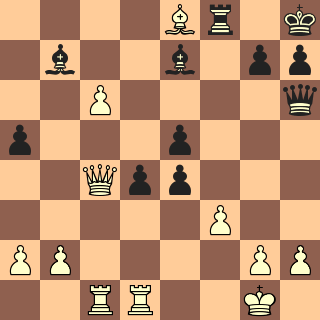
\includegraphics[scale=0.5]{fig/diagram_feat}
\caption[Chess Position]{chess position coming out of the game \textit{Alexander McDonnell vs Louis Charles Mahe De La Bourdonnais, London 1834} after 24. c6}
\label{fig:feat}
\end{figure}

\begin{table}[]
\centering
\begin{tabular}{c c c | c c c}
\toprule
\textbf{piece} & \textbf{piece map} & \textbf{mobility map} & \textbf{piece} & \textbf{piece map} & \textbf{mobility map} \\
\midrule

\includegraphics[scale=0.5]{fig/pieces/K} & 
$ \begin{smallmatrix} 0&0&0&0&0&0&0&0\\0&0&0&0&0&0&0&0\\0&0&0&0&0&0&0&0\\0&0&0&0&0&0&0&0\\0&0&0&0&0&0&0&0\\0&0&0&0&0&0&0&0\\0&0&0&0&0&0&0&0\\0&0&0&0&0&0&1&0 \end{smallmatrix} $ &  $\begin{smallmatrix}0&0&0&0&0&0&0&0\\0&0&0&0&0&0&0&0\\0&0&0&0&0&0&0&0\\0&0&0&0&0&0&0&0\\0&0&0&0&0&0&0&0\\0&0&0&0&0&0&0&0\\0&0&0&0&0&1&0&0\\0&0&0&0&0&1&0&1\end{smallmatrix}$  &


\includegraphics[scale=0.5]{fig/pieces/k} &
$\begin{smallmatrix}0&0&0&0&0&0&0&1\\0&0&0&0&0&0&0&0\\0&0&0&0&0&0&0&0\\0&0&0&0&0&0&0&0\\0&0&0&0&0&0&0&0\\0&0&0&0&0&0&0&0\\0&0&0&0&0&0&0&0\\0&0&0&0&0&0&0&0\end{smallmatrix}$ &
$\begin{smallmatrix}0&0&0&0&0&0&0&0\\0&0&0&0&0&0&0&0\\0&0&0&0&0&0&0&0\\0&0&0&0&0&0&0&0\\0&0&0&0&0&0&0&0\\0&0&0&0&0&0&0&0\\0&0&0&0&0&0&0&0\\0&0&0&0&0&0&0&0\end{smallmatrix}$ \\ [1cm]


\includegraphics[scale=0.5]{fig/pieces/Q} & 
$\begin{smallmatrix}0&0&0&0&0&0&0&0\\0&0&0&0&0&0&0&0\\0&0&0&0&0&0&0&0\\0&0&0&0&0&0&0&0\\0&0&1&0&0&0&0&0\\0&0&0&0&0&0&0&0\\0&0&0&0&0&0&0&0\\0&0&0&0&0&0&0&0\end{smallmatrix}$ &
$\begin{smallmatrix}0&0&0&0&0&0&1&0\\0&0&0&0&0&1&0&0\\1&0&0&0&1&0&0&0\\0&1&1&1&0&0&0&0\\1&1&0&1&0&0&0&0\\0&1&1&1&0&0&0&0\\0&0&1&0&1&0&0&0\\0&0&0&0&0&1&0&0\end{smallmatrix}$&


\includegraphics[scale=0.5]{fig/pieces/q} &
$\begin{smallmatrix}0&0&0&0&0&0&0&0\\0&0&0&0&0&0&0&0\\0&0&0&0&0&0&0&1\\0&0&0&0&0&0&0&0\\0&0&0&0&0&0&0&0\\0&0&0&0&0&0&0&0\\0&0&0&0&0&0&0&0\\0&0&0&0&0&0&0&0\end{smallmatrix}$ &
$\begin{smallmatrix}0&0&0&0&0&0&0&0\\0&0&0&0&0&0&0&0\\0&0&1&1&1&1&1&0\\0&0&0&0&0&0&1&1\\0&0&0&0&0&1&0&1\\0&0&0&0&1&0&0&1\\0&0&0&1&0&0&0&1\\0&0&1&0&0&0&0&0\end{smallmatrix}$ \\ [1cm]


\includegraphics[scale=0.5]{fig/pieces/R} & 
$\begin{smallmatrix}0&0&0&0&0&0&0&0\\0&0&0&0&0&0&0&0\\0&0&0&0&0&0&0&0\\0&0&0&0&0&0&0&0\\0&0&0&0&0&0&0&0\\0&0&0&0&0&0&0&0\\0&0&0&0&0&0&0&0\\0&0&1&1&0&0&0&0\end{smallmatrix}$ &
$\begin{smallmatrix}0&0&0&0&0&0&0&0\\0&0&0&0&0&0&0&0\\0&0&0&0&0&0&0&0\\0&0&0&0&0&0&0&0\\0&0&0&1&0&0&0&0\\0&0&1&1&0&0&0&0\\0&0&1&1&0&0&0&0\\1&1&0&0&1&1&0&0\end{smallmatrix}$ &

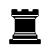
\includegraphics[scale=0.5]{fig/pieces/r} &
$\begin{smallmatrix}0&0&0&0&0&1&0&0\\0&0&0&0&0&0&0&0\\0&0&0&0&0&0&0&0\\0&0&0&0&0&0&0&0\\0&0&0&0&0&0&0&0\\0&0&0&0&0&0&0&0\\0&0&0&0&0&0&0&0\\0&0&0&0&0&0&0&0\end{smallmatrix}$ &
$\begin{smallmatrix}0&0&0&0&1&0&1&0\\0&0&0&0&0&1&0&0\\0&0&0&0&0&1&0&0\\0&0&0&0&0&1&0&0\\0&0&0&0&0&1&0&0\\0&0&0&0&0&1&0&0\\0&0&0&0&0&0&0&0\\0&0&0&0&0&0&0&0\end{smallmatrix}$ \\ [1cm]


\includegraphics[scale=0.5]{fig/pieces/B} & 
$\begin{smallmatrix}0&0&0&0&1&0&0&0\\0&0&0&0&0&0&0&0\\0&0&0&0&0&0&0&0\\0&0&0&0&0&0&0&0\\0&0&0&0&0&0&0&0\\0&0&0&0&0&0&0&0\\0&0&0&0&0&0&0&0\\0&0&0&0&0&0&0&0\end{smallmatrix}$&
$\begin{smallmatrix}0&0&0&0&0&0&0&0\\0&0&0&1&0&1&0&0\\0&0&0&0&0&0&1&0\\0&0&0&0&0&0&0&1\\0&0&0&0&0&0&0&0\\0&0&0&0&0&0&0&0\\0&0&0&0&0&0&0&0\\0&0&0&0&0&0&0&0\end{smallmatrix}$ &


\includegraphics[scale=0.5]{fig/pieces/b} &
$\begin{smallmatrix}0&0&0&0&0&0&0&0\\0&1&0&0&1&0&0&0\\0&0&0&0&0&0&0&0\\0&0&0&0&0&0&0&0\\0&0&0&0&0&0&0&0\\0&0&0&0&0&0&0&0\\0&0&0&0&0&0&0&0\\0&0&0&0&0&0&0&0\end{smallmatrix}$&
$\begin{smallmatrix}1&0&1&1&0&0&0&0\\0&0&0&0&0&0&0&0\\1&0&1&1&0&1&0&0\\0&0&1&0&0&0&1&0\\0&1&0&0&0&0&0&1\\1&0&0&0&0&0&0&0\\0&0&0&0&0&0&0&0\\0&0&0&0&0&0&0&0\end{smallmatrix}$ \\ [1cm]


\includegraphics[scale=0.5]{fig/pieces/N} &
$\begin{smallmatrix}0&0&0&0&0&0&0&0\\0&0&0&0&0&0&0&0\\0&0&0&0&0&0&0&0\\0&0&0&0&0&0&0&0\\0&0&0&0&0&0&0&0\\0&0&0&0&0&0&0&0\\0&0&0&0&0&0&0&0\\0&0&0&0&0&0&0&0\end{smallmatrix}$&
$\begin{smallmatrix}0&0&0&0&0&0&0&0\\0&0&0&0&0&0&0&0\\0&0&0&0&0&0&0&0\\0&0&0&0&0&0&0&0\\0&0&0&0&0&0&0&0\\0&0&0&0&0&0&0&0\\0&0&0&0&0&0&0&0\\0&0&0&0&0&0&0&0\end{smallmatrix}$ &


\includegraphics[scale=0.5]{fig/pieces/n} &
$\begin{smallmatrix}0&0&0&0&0&0&0&0\\0&0&0&0&0&0&0&0\\0&0&0&0&0&0&0&0\\0&0&0&0&0&0&0&0\\0&0&0&0&0&0&0&0\\0&0&0&0&0&0&0&0\\0&0&0&0&0&0&0&0\\0&0&0&0&0&0&0&0\end{smallmatrix}$ &
$\begin{smallmatrix}0&0&0&0&0&0&0&0\\0&0&0&0&0&0&0&0\\0&0&0&0&0&0&0&0\\0&0&0&0&0&0&0&0\\0&0&0&0&0&0&0&0\\0&0&0&0&0&0&0&0\\0&0&0&0&0&0&0&0\\0&0&0&0&0&0&0&0\end{smallmatrix}$ \\ [1cm]


\includegraphics[scale=0.5]{fig/pieces/P} &
$\begin{smallmatrix}0&0&0&0&0&0&0&0\\0&0&0&0&0&0&0&0\\0&0&1&0&0&0&0&0\\0&0&0&0&0&0&0&0\\0&0&0&0&0&0&0&0\\0&0&0&0&0&1&0&0\\1&1&0&0&0&0&1&1\\0&0&0&0&0&0&0&0\end{smallmatrix}$ &
$\begin{smallmatrix}0&0&0&0&0&0&0&0\\0&1&1&0&0&0&0&0\\0&0&0&0&0&0&0&0\\0&0&0&0&0&0&0&0\\1&1&0&0&1&1&1&1\\1&1&0&0&0&0&1&1\\0&0&0&0&0&0&0&0\\0&0&0&0&0&0&0&0\end{smallmatrix}$ &

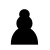
\includegraphics[scale=0.5]{fig/pieces/p} &
$\begin{smallmatrix}0&0&0&0&0&0&0&0\\0&0&0&0&0&0&1&1\\0&0&0&0&0&0&0&0\\1&0&0&0&1&0&0&0\\0&0&0&1&1&0&0&0\\0&0&0&0&0&0&0&0\\0&0&0&0&0&0&0&0\\0&0&0&0&0&0&0&0\end{smallmatrix}$ &
$\begin{smallmatrix}0&0&0&0&0&0&0&0\\0&0&0&0&0&0&0&0\\0&0&0&0&0&0&1&0\\0&0&0&0&0&0&1&0\\1&0&0&0&0&0&0&0\\0&0&0&1&1&1&0&0\\0&0&0&0&0&0&0&0\\0&0&0&0&0&0&0&0\end{smallmatrix}$ \\

\bottomrule
\end{tabular}
\caption[Bitboards]{An example of how the chessboard from figure \ref{fig:feat} can be transformed to a stack of binary image channels}
\label{tab:feat}
\end{table}


\label{ex:feat}

Next to this, we can add additional (redundant) information to the features to help the model in question to learn patterns. Examples of additional features are
\begin{itemize}
\item side to move
\item indication for each castle if it is still possible
\item possibility to do en passant for each of the 16 squares where this could be a possibility
\item piece count for each piece type
\item piece mobility: number of squares each piece can go to
\item for each piece (type) the number of pieces it attacks
\item for each piece (type) the number of pieces it defends
\end{itemize}
We will call this data global features from now on. Some of these could be encoded with image maps as well. For example, every cell could denote the number of times it is attacked and defended.

\section{Static Evaluation Function}
\label{sec:sef}
In conventional chess engines, the heuristic evaluation function is linear, but also reinforcement learning chess programs often use a linear function: $V_w(s)=\sum w f(s)$ \cite{baxt99,veness09}. In this dissertation, we switch gears and use a neural network model instead, as they have the ability to model a larger range of functions and extract additional features from the data.\\
The chess engine \textit{Giraffe}, which uses a TD-learning algorithm, uses an \gls{fnn} architecture with 2 hidden layers \cite{giraffe15}. A totally different approach has been taken in \textit{DeepChess}, where the evaluation function is a deep siamese network learned on a big dataset of games between grandmasters. Two positions are given as input and the network returns which position is best. Playing is then performed with a comparison-based $\alpha\beta$-search. Admirably, \textit{DeepChess} succeeded at reaching a grandmaster level of play \cite{David2016}.\\

To our best knowledge, no one has experimented with a \gls{cnn} architecture to evaluate chess positions yet. The feature space presented in the previous section forms an intuitive basis to start with. The distinction between bitboard and global features demands for an architecture where the channel stack is the input of a \gls{cnn}, where some form of feature extraction is carried out. Next, the resulting feature maps are combined with the global feature vector into a \gls{fcn} with regression, as shown in figure \ref{fig:chessnetw}. 

\begin{figure}
\centering
\begin{tikzpicture}[scale=0.75]
%\draw[step=0.5cm,gray,very thin] (0,-4) grid (20,4);
\node (img) at (1,0) {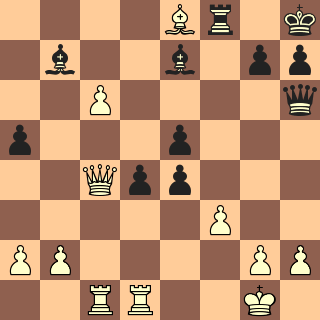
\includegraphics[width=1.6cm]{fig/diagram_feat}};
\node at (-0.5,0) {$s$};
\draw (3,1.5) rectangle (5,3.5);
\draw (3.5,2) rectangle (5.5,4);
\draw (3.25,1.75) rectangle (5.25,3.75);
\draw[->] (1,1) -- (1,2.5) -- (3,2.5);
\draw (4,-1.5) rectangle (4.5,-4);
\draw[->] (1,-1) -- (1,-2.75) -- (4,-2.75);
\node at (4.25,1.25){bitboards};
\node at (3.25,-2.5){global};

\draw[->] (5.5,2.5) -- (7.5,2.5);
\draw (7.5,1.5) rectangle (10.5,3.5) node[pos=0.5,scale=2]{CNN};

\draw[->] (10.5,2.5) -- (12.5,2.5);
\draw (12.5,1.5) rectangle (14.5,3.5);
\draw (13,2) rectangle (15,4);
\draw (12.75,1.75) rectangle (14.75,3.75);
\node at (13.75,1.25){feature maps};

\draw[->] (15,2.5) -- (17,2.5);
\draw[->] (4.5,-2.75) -- (17,-2.75);
\draw[->] (17,-4) rectangle (18.5,4);
\node[scale=2.5] at (17.75,1.25) {F};
\node[scale=2.5] at (17.75,0) {C};
\node[scale=2.5] at (17.75,-1.25) {N};

\draw[->] (18.5,0) -- (20.5,0) node[pos=0.5,yshift=7.5pt]{$V(s)$};

%\node[staterect] (n0_0) at (0,0) {Agent} edge[mainedge, bend left] (n0_4);
%\node[staterect] (n0_4) at (0,-4) {Environment: $s_t$} edge[mainedge, bend left] (n0_0);
%\node at (-1,-2) {$a_t$};
%\node at (1.1,-2) {$r_{t+1}$};
%\node at (1.1,-2.5) {$s_{t+1}$};
\end{tikzpicture}
\caption[Network architecture value function]{Schematic overview of a possible network architecture for chess using CNNs}
\label{fig:chessnetw}
\end{figure}

\section{TD algorithms}
\label{sec:td}
As investigated in section \ref{subsec:vp}, TD algorithms are ideal in a \acrlong{ml} framework, because of its natural embedding of the optimization of the \gls{mse} cost function in its update rule. We saw that a TD($\lambda$) approach is often the best choice, as it combines the best of both \gls{mc} methods and classical \gls{td}-learning. We shortly review \gls{td}($\lambda$) in section \ref{subsec:tdy} and analyze its shortcomings, after which we consider alternatives using both the ideas of \gls{td}($\lambda$) and minimax search (for which it is of course more efficient to apply the $\alpha\beta$-search). These methods slightly differ in terms of the episodic weight updates.\\

Before we continue, we need to revise the \gls{rl} framework. In literature, the \gls{rl} framework for boardgames is often a simplification of the classical one represented in section \ref{sec:rl}. The reward function $r:\mathcal{S}\times\mathcal{A}\mapsto \mathbb{R}$ in boardgames is often chosen to be
\begin{equation}
\label{eq:reward}
r(s_t,a_t) = \begin{cases} 
   W(s_{t+1}) & \text{if } s_{t+1} \textnormal{ is terminal} \\
   0 & \text{if } \textnormal{else}
  \end{cases}
\end{equation}
where $W(s_{t+1})$ denotes the objective evaluation of the terminal state of the game (do not confuse with the static evaluation function). For chess, this objective evaluation can be (assuming $s$ is a terminal state)
\begin{equation}
W(s) = \begin{cases} 
   1 & \text{win} \\
   0 & \text{draw} \\
   -1 & \text{loss} \\
  \end{cases}
\end{equation}
Notice how this definition of the reward function meets the zero sum property. \\
Previous research in \gls{rl} in games mainly do not take the discount factor into account when performing a TD-learning. This is rationalized by considering the return $\mathcal{R}=\sum_{t=0}^{T}\gamma^t r(s_t,a_t)$. As $r(s_t,a_t)$ is zero everywhere except at the final state, it may be beneficial to assign the final reward as the return of every action, especially in \gls{td}-learning algorithms. The reason for this is a remark made in section \ref{subsec:vp} about the otherwise slow convergence properties in chaining.\\

In what follows, we will consider two main ideas to compute a target:
\begin{itemize}
\item episodic updates of the weights. After each episode the weights can be updated with an update rule. We could say this is a way of doing incremental learning over episodes. Here it is important to notice that the updates are heavily correlated, which may be the cause of bad generalization if we were to use them incrementally. The update rules make use of the assumptions about the simplified reward function and neutralized discount factor.
\item translation to supervised learning framework. What is needed, are a set of tuples $(s,\mathcal{R})$ where the return operates as a target value to learn $V(s)$. By using this approach, we can choose our favorite supervised learning algorithm from section \ref{subsubsec:ann}. We can gather these tuples over the course of many episodes and shuffle them before applying mini-batch \gls{sgd} (which is in general beneficial for the performance in software implementations) to improve generalization. 
\end{itemize}

\subsection{TD($\lambda$)}
\label{subsec:tdy}
\gls{td}($\lambda$) was the first \gls{rl} algorithm that proved to effective for learning to play a game. \textit{TD-Gammon} used a \acrlong{nn} with one fully connected sigmoidal hidden layer to learn a value function for backgammon \cite{tdgammon95}. Assume from now on  

\begin{equation}
V_{est}(s_t)=\begin{cases} 
   r_t &  \text{if } t=T \\
   \hat{V}(s_t) & \text{else} \\
  \end{cases}
\end{equation}

Under the conditions $\gamma=0$ and equation \ref{eq:reward} the temporal difference is defined to be

\begin{equation}
\label{eq:td}
\delta_t=V_{est}(s_{t+1})-V_{est}(s_{t})
\end{equation}

If we use a learning rate $\alpha$, we can now update the parameters after each episode with a history $(s_0,a_0,r_1),(s_1,a_1,r_2), \dotso , (s_{T-1},a_{T-1},r_T)$ as follows:

\begin{equation}
\label{eq:update}
w \leftarrow w-\alpha \sum_{t=0}^{T-1} \nabla_w V_{est}(s_t) \sum_{n=t}^{T-1} \lambda^{n-t}\delta_n
\end{equation}

This is equivalent to an episodic gradient descent update minimizing the \gls{mse} with the $\lambda$-return as target in supervised learning context. Remember that the general regression supervised learning paradigm can be summarized for a target $z$ with the formula

\begin{equation}
\bigtriangleup w =\alpha \nabla_w V_{est}(s_t) (z_t-V_{est}(s_t))
\end{equation}

Over the course of an episode $\left[s_0,r_1,s_1,\dotso,r_T,s_T\right]$, the total update amounts to
\begin{equation}
\bigtriangleup w =\alpha \sum_{t=0}^{T-1} \nabla_w V_{est}(s_t) (z_t-V_{est}(s_t))
\end{equation}
Hence, if equation \ref{eq:update} were a gradient descent update, following equality should hold:
\begin{equation}
z_t-V_{est}(s_t) = \sum_{n=t}^{T-1} \lambda^{n-t}\delta_n
\end{equation}
Working this out yields
\begin{align*}
z_t &=\sum_{n=t}^{T-1} \lambda^{n-t} \left[V_{est}(s_{n+1})-V_{est}(s_{n})\right]+V_{est}(s_t) \\
&= \quad \quad \lambda^0\left[V_{est}(s_{t+1}-V_{est}(s_t))\right] \\
& \quad \quad+\lambda\left[V_{est}(s_{t+2}-V_{est}(s_{t+1}))\right] \\
& \quad \quad+ \dotso\\
& \quad \quad +\lambda^{T-1-t}\left[V_{est}(s_{T}-V_{est}(s_{T-1}))\right] + V_{est}(s_T) \\
&= \sum_{n=0}^{T-2-t}(\lambda^n-\lambda^{n+1})V_{est}(s_{t+1+n}) \lambda^{T-1-t}V_{est}(s_T)\\
&= (1-\lambda)\sum_{n=1}^{T-1-t}\lambda^{n-1}V_{est}(s_{t+n}) + \lambda^{T-1-t}V_{est}(s_T)\\
&= (1-\lambda)\sum_{n=1}^{T-1-t}\lambda^{n-1}V_{est}(s_{t+n}) + \lambda^{T-1-t}(1-\lambda)V_{est}(s_T)+ \lambda^{T-t}V_{est}(s_T)\\
&= (1-\lambda)\sum_{n=1}^{T-t}\lambda^{n-1}V_{est}(s_{t+n}) + \lambda^{T-t}V_{est}(s_T)\\
\end{align*}
Combining the defined reward function, $\gamma=1$ and equation \ref{eq:nstep} for the n-step return, we notice how the n-step return is equal to the approximated value function n steps ahead: $G_n(s_t)=V_{est}(s_{t+n})$. The return after the terminal state is trivially estimated to be the value function at the terminal state: $V(s_T)$. Hence we achieve (using equation \ref{eq:tdlambda_fin}) our final result
\begin{align}
z_t&=(1-\lambda)\sum_{n=0}^{T-t}\lambda^{n-1}G_n(s_t) + G_t\\
&=G_\lambda(s_t)
\end{align}

The amazing thing about \textit{TD-Gammon} is that its level surpassed that of humans by using strategies that were considered bad at that time. These techniques were later incorporated into humans play. One characteristic about its evaluations was that objectively better positions were estimated a smaller value than worse positions. Still, the engine was able to choose the best move. \textit{Tesauro} explains this by the huge similarity between consecutive positions for the neural network, resulting in a smaller difference. For choosing the right move, the relative error is much more important than the absolute error.\\
Another key to the success of \textit{TD-Gammon} is the stochasticity of the game. Thanks to the stochastic noise the agent is able to discover new strategies much quicker than it would in a deterministic environment.\\

In section \ref{subsec:vp} a supervised learning algorithm using $z_t$ as target was laid out. It is key to remember that the update rule from equation \ref{eq:update} is essentially a supervised learning regression algorithm, but generalizing for $G_lambda(s_t)$ may be beneficial, as we can study the influence of the discount factor and reward function in this manner. To resume and summarize, the target values for the network are equal to

\begin{equation}
G_\lambda(s_t) = (1-\lambda) \sum_{n=1}^{T-t} \lambda^{n-1} \left[\sum_{i=0}^{n-1} \left( \gamma^i r_{k+i}\right) + \gamma^n V_{est}(s_{k+n}) \right]
\end{equation}

in the standard TD($\lambda$) method. The techniques from the following sections will only differ in how we define our target $z_t=G_\lambda(s_t)$.\\
Algorithm \ref{al:sltd} is the supervised learning framework, independent of the definition of $z_t$, hence independent of the implemented \gls{td} algorithm and conditions. It consists of following noteworthy elements:
\begin{itemize}
\item random initialization of the network's parameters.
\item playing episodes with the current network under some policy. Let us assume it is $\epsilon$-greedy for now.
\item calculating the matching returns from all played games and adding the tuples $(s_t,z_t)$ to replay memory $\mathcal{D}$. In algorithm \ref{al:sltd} the replay memory gets refreshed every iteration, but more sophisticated methods to have a representable dataset may be applied.
\item splitting $\mathcal{D}$ in a training set $\mathcal{D}_{training}$ and validation set $\mathcal{D}_{test}$
\item doing experience replay: random sampling of minibatches from $\mathcal{D}$, from which the weights will be updated with gradient descent.
\item learn until the loss on the validation set stops decreasing, to avoid the network from overfitting.
\end{itemize}

\begin{algorithm}
\begin{algorithmic}
	\STATE Initialize $w$ (randomly)
	\REPEAT
		\STATE play $N$ episodes $\rightarrow (\mathcal{H}_1,\dotso,\mathcal{H}_N)$
		\STATE $\mathcal{D}=\{\}$
		\COMMENT{create a dataset to store experience from episodes}
		\FOR {$i\leftarrow 1$ to $N$}
			\FOR {$s_t \in \mathcal{H}_i$}
				\STATE$\mathcal{D} \leftarrow \mathcal{D} \cup \{(s_t,z_t)\}$
				\COMMENT{calculate return}
			\ENDFOR
		\ENDFOR
		\STATE shuffle samples
		\STATE select $\mathcal{D}_{training}$ and $\mathcal{D}_{test}$ from  $\mathcal{D}$
		\REPEAT		
			\FOR{all minibatches $\in \mathcal{D}_{training}$}
				\STATE $w \gets w-\alpha\sum_{i=1}^{n}\frac{\nabla L_i(w)}{n}$
			\ENDFOR
		\UNTIL loss on $\mathcal{D}_{test}$ stops decreasing
	\UNTIL satisfying convergence
\end{algorithmic}
\caption{supervised TD algorithm}
\label{al:sltd}
\end{algorithm}

If we were to implement TD($\lambda$) onto the chess model, it would be hard for the agent to learn to play well. This is due to these main reasons:
\begin{itemize}
\item in contrast to backgammon, chess is a deterministic game, which will make exploration harder under a non adapted policy
\item chess is a very tactical game. This fact requires some sort of tree search. With TD($\lambda$) we are only looking one move ahead under an $\epsilon$-greedy policy.
\end{itemize}
The policy problem is somewhat hard to solve (we will look further into it in section \ref{sec:polnet}), but we can introduce tree search in different fashions as we will see next. 

\subsection{TD-directed($\lambda$)}
\label{subsec:tddir}
This is the easiest minimax variant proposed by the developers of \textit{KnightCap} \cite{baxt99}. The same update rules and target are applied as in TD($\lambda$). The one difference lies in the policy. Play is guided by the minimax value at a depth $d$.

\subsection{TD-root($\lambda$)}
\label{subsec:tdroot}
A first algorithm introducing a minimax search into TD-learning is TD-root($\lambda$), its idea already dates back to 1959(!), where the agent was able to reach an amateur level in checkers \cite{samuel59}. The idea is to update the value functions in positions into the direction of the minimax values, as they are better representation of the actual value at that state, as shown in figure \ref{fig:tdroot}. By doing this, the values at states will have the tree search incorporated into it. The value at the roots change into the direction of the values at the leafs of the principal variations.\\
To continue, we define the function $l:\mathcal{S} \times \mathbb{N}_{>0}\mapsto\mathcal{S}$ that projects a state to its leaf state given a depth following the path of the \acrlong{pv}. To incorporate this idea into \gls{td} learning, we only need to slightly modify equation \ref{eq:td} for a certain depth $d$ to 
\begin{equation}
\label{eq:tdroot}
\delta_t=V_{est}\left(l(s_{t+1},d)\right)-V_{est}(s_{t})
\end{equation}
The update rule with the simplified conditions and TD-error from equation \ref{eq:tdroot} is then equation \ref{eq:update}. The corresponding target value for every state is consequently
\begin{equation}
z_t=\sum_{n=t}^{T-1} \lambda^{n-t} \delta_n+V_{est}(s_T)
\end{equation}

\begin{figure}
\centering
\begin{tikzpicture}[scale=0.9]
%\draw[step=1cm,gray,very thin] (-8,-2) grid (8,4);
\node[state,fill=black] (s0) at (-5,4){} ;
\node[state] (s1) at (-7,2){} edge[mainedge,dashed] (s0);
\node[state] (s2) at (-3,2){} edge[mainedge] (s0);
\node[state] (s3) at (-8,0){} edge[mainedge,dashed] (s1);
\node[state] (s4) at (-6,0){} edge[mainedge,dashed] (s1);
\node[state] (s5) at (-4,0){} edge[mainedge] (s2);
\node[state] (s6) at (-2,0){} edge[mainedge,dashed] (s2);
\node at (-5,-1){$t$};

\draw[dashed] (0,-1) -- (0,5);

\node[state,fill=blue] (t0) at (5,4){};
\node[state] (t1) at (7,2){} edge[mainedge,dashed] (t0);
\node[state] (t2) at (3,2){} edge[mainedge] (t0);
\node[state] (t3) at (8,0){} edge[mainedge,dashed] (t1);
\node[state] (t4) at (6,0){} edge[mainedge,dashed] (t1);
\node[state] (t5) at (4,0){} edge[mainedge,dashed] (t2);
\node[state,fill=red] (t6) at (2,0){} edge[mainedge] (t2);
\node at (5,-1){$t+1$};

\node[state] (s0) at (-5,4){} edge[mainedge,color=red,bend left] node[midway,xshift=-0.5cm,yshift=-0.5cm]{TD-root($\lambda$)} (t6) edge[mainedge,color=blue,bend left=10] node[midway,yshift=-0.5cm]{TD($\lambda$)} (t0);

\end{tikzpicture}
\caption[Comparison between TD-root($\lambda$) and TD($\lambda$)]{Comparison between TD-root($\lambda$) and TD($\lambda$). In TD($\lambda$), the root nodes get feedback (an error signal) from the root at the next time step, while in TD-root($\lambda$), the root receives its feedback signal from the principal leaf node at the next state.}
\label{fig:tdroot}
\end{figure}

\subsection{TD-leaf($\lambda$)}
\label{subsec:tdleaf}
An issue with TD($\lambda$) and TD-root($\lambda$) is that they only update according the line of play, which correlates the data. By using the same minimax idea as before, but now updating the leaf along the \gls{pv} to the leaf along the \gls{pv} of the next position, we obtain data from positions not played. This is because the \gls{pv} up until a certain depth is not necessarily the same path as in the following position. This idea is named TD-leaf($\lambda$), and was used to train against expert chess opponents in \textit{KnightCap} and \textit{Giraffe} \cite{baxt99,giraffe15}. Also with TD-leaf($\lambda$), a superhuman level in checkers has been achieved \cite{chinook}. The update rule is depicted at figure \ref{fig:tdleaf}. \\
The temporal difference and corresponding update rule defining this update are
\begin{align}
\delta_t&=V_{est}\left(l(s_{t+1},d)\right)-V_{est}(l(s_{t},d))\\
w &\leftarrow w-\alpha \sum_{t=0}^{T-1} \nabla_w V_{est}(l(s_t,d)) \sum_{n=t}^{T-1} \lambda^{n-t}\delta_n
\end{align}
Hence, our tuple for our supervised learning framework consists out of $l(s_t)$ and
\begin{equation}
z_t=\sum_{n=t}^{T-1} \lambda^{n-t} \delta_n+V_{est}(l(s_T,d))
\end{equation}
which analogously as in section \ref{subsec:tdy} can be transformed to
\begin{align}
z_t&=(1-\lambda)\sum_{n=0}^{T-t}\lambda^{n-1}V_{est}(l(s_{t+n},d)) + \lambda^{T-t}V_{est}(s_T)\\
&=G_\lambda(s_t)
\label{eq:leafreturn}
\end{align}
using the property that the leaf of a terminal state is itself, or put otherwise $l(s_T)=s_T$. With equation \ref{eq:leafreturn}, we can define the $\lambda$-return for general discount rates and reward functions.
The attentive reader noticed it was impossible to generalize the target to $G_\lambda(s_t)$ for TD-root($\lambda$), because factors can not be canceled out when comparing leaves to roots.

\begin{figure}
\centering
\begin{tikzpicture}[scale=0.9]
%\draw[step=1cm,gray,very thin] (-8,-2) grid (8,4);
\node[state] (s0) at (-5,4){} ;
\node at (-4.25,4){$s_t$};
\node[state] (s1) at (-7,2){} edge[mainedge,dashed] (s0);
\node[state] (s2) at (-3,2){} edge[mainedge] (s0);
\node at (-2.125,2){$s_{t+1}$};
\node[state] (s3) at (-8,0){} edge[mainedge,dashed] (s1);
\node[state] (s4) at (-6,0){} edge[mainedge,dashed] (s1);
\node[state,fill=black] (s5) at (-4,0){} edge[mainedge] (s2);
\node[state] (s6) at (-2,0){} edge[mainedge,dashed] (s2);
\node at (-5,-1){$t$};

\draw[dashed] (0,-1) -- (0,5);

\node[state] (t0) at (5,4){};
\node at (5.875,4){$s_{t+1}$};
\node[state] (t1) at (7,2){} edge[mainedge,dashed] (t0);
\node[state] (t2) at (3,2){} edge[mainedge] (t0);
\node[state] (t3) at (8,0){} edge[mainedge,dashed] (t1);
\node[state] (t4) at (6,0){} edge[mainedge,dashed] (t1);
\node[state] (t5) at (4,0){} edge[mainedge,dashed] (t2);
\node[state,fill=black] (t6) at (2,0){} edge[mainedge] (t2);
\node at (5,-1){$t+1$};

\node[state] (s0) at (-4,0){} edge[mainedge,color=black,bend right=20] node[midway,yshift=-0.5cm]{TD-leaf($\lambda$)} (t6);

\end{tikzpicture}
\caption[TD-leaf($\lambda$)]{How updates in TD-leaf($\lambda$) work. The \gls{pv}s are denoted by the non dashed paths in the search tree. Notice how the paths may be different in the next state. The updates happen from leaf to leaf, which not necessary need to be played.}
\label{fig:tdleaf}
\end{figure}

\subsection{TD-stem($\lambda$)}
\label{subsec:tdrootleaf}
To conclude this section about TD algorithms, we will examine an own contribution (to the best of our knowledge): TD-stem($\lambda$). The idea is to simply combine the ideas of TD-leaf($\lambda$) and TD-root($\lambda$) by defining the error as the difference between the leaves, but updating the root state. This makes sense, as it seems to annihilate disadvantages of the former methods. In TD-leaf($\lambda$) the update can be from another path (resulting in being erroneous), while TD-root($\lambda$) can not be generalized to a $\lambda$-return. Essentially, the update is in the direction of the error between the minimax values of consecutive states. An additional bonus could be the incorporation of depth into the static evaluation function. However, this could also be a disadvantage, as this could make the evaluation more noisy. the main idea is depicted in \ref{fig:tdrootleaf}. \\
To formalize this idea into mathematics:
\begin{align}
\delta_t&=V_{est}\left(l(s_{t+1},d)\right)-V_{est}(l(s_{t},d))\\
w &\leftarrow w-\alpha \sum_{t=0}^{T-1} \nabla_w V_{est}(s_t) \sum_{n=t}^{T-1} \lambda^{n-t}\delta_n
\end{align}
The generalization to $\lambda$-return is straightforward, with retrospect to equation \ref{eq:leafreturn}.

\begin{figure}
\centering
\begin{tikzpicture}[scale=0.9]
%\draw[step=1cm,gray,very thin] (-8,-2) grid (8,4);
\node[state,fill=black] (s0) at (-5,4){} ;
\node at (-4.25,4){};
\node[state] (s1) at (-7,2){} edge[mainedge,dashed] (s0);
\node[state] (s2) at (-3,2){} edge[mainedge] (s0);
\node at (-2.125,2){};
\node[state] (s3) at (-8,0){} edge[mainedge,dashed] (s1);
\node[state] (s4) at (-6,0){} edge[mainedge,dashed] (s1);
\node[state,fill=black] (s5) at (-4,0){} edge[mainedge] (s2);
\node[state] (s6) at (-2,0){} edge[mainedge,dashed] (s2);
\node at (-5,-1){$t$};

\draw[dashed] (0,-1) -- (0,5);

\node[state] (t0) at (5,4){};
\node at (5.875,4){};
\node[state] (t1) at (7,2){} edge[mainedge,dashed] (t0);
\node[state] (t2) at (3,2){} edge[mainedge] (t0);
\node[state] (t3) at (8,0){} edge[mainedge,dashed] (t1);
\node[state] (t4) at (6,0){} edge[mainedge,dashed] (t1);
\node[state] (t5) at (4,0){} edge[mainedge,dashed] (t2);
\node[state,fill=black] (t6) at (2,0){} edge[mainedge] (t2);
\node at (5,-1){$t+1$};

\node[state] (s0) at (-4,0){} edge[mainedge,color=black,bend right=20](t6);
\node[state] (s1) at (-5,4){} edge[mainedge,color=black] node[midway,xshift=-0.9cm,yshift=-0.5cm]{TD-stem($\lambda$)} (s0);

\end{tikzpicture}
\caption[TD-stem($\lambda$)]{In TD-stem($\lambda$), the root is updated based on values of the consecutive leaf node values.}
\label{fig:tdrootleaf}
\end{figure}

\section{Bootstrapping Tree Search}
\label{sec:bts}
There are three drawbacks to the TD algorithms with search included discussed in previous section:
\begin{enumerate}
\item Only one node gets updated for every tree search, making the search somewhat inefficient.
\item The positions may not be representative or too coherent with each other, as they are all based on actual occurrences or computed best line of play (\gls{pv}).
\item The target search is based on move played. Hence, this method is much more effective when the player is already strong.
\end{enumerate}
Especially the third point is a major turn off in our point of view, as we want to inject as less expert domain knowledge as possible into our model.\\
To address these problems, we could make more samples by using all information we got from the tree search. Additionally, we do not use the search from future, but rather use the minimax value directly as target. These ideas have been implemented in the chess engine \textit{Meep}, reaching an expert rating with self play \cite{veness09}.

%
%\subsection{Rootstrap($\lambda$)}
%\label{subsec:rootstrap}
%In rootstrap, the supervised learning framework can be used. The tuple consists out of the state from self-play $s_t$ and the estimated value at the leaf node:
%\begin{equation}
%z_t=V_{est}(l(s_t))
%\end{equation}
%This is the way it was implemented in \textit{Meep}, but we can actually generalize this to also include temporal knowledge into our target by using ideas from \gls{td} learning as we have seen in section \ref{sec:td} in the following way:
%\begin{align}
%\delta_t&=V_{est}(l(s_t,d))-V_{est}(s_t) \\
%z_t&=\sum_{n=t}^{T-1} \lambda^{n-t} \delta_n+V_{est}(l(s_T,d))
%\end{align}
%The corresponding change of the parameters over the course of an episode would then be
%\begin{equation}
%\bigtriangleup w =\alpha \sum_{t=0}^{T-1}\nabla_w V_{est}(s_t) \sum_{n=t}^{T-1} \lambda^{n-t} \delta_n
%\end{equation}
%By reformulating this equation
%\begin{align*}
%\bigtriangleup w &=\alpha \sum_{t=0}^{T-1}\nabla_w V_{est}(s_t) \sum_{n=t}^{T-1} \lambda^{n-t} \left[V_{est}(l(s_n,d))-V_{est}(s_{n+1})\right] \\
%&= \alpha \sum_{n=0}^{T-1} \left[V_{est}(l(s_n,d))-V_{est}(s_{n+1})\right] \sum_{t=0}^{n} \lambda^{n-t} \nabla_w V_{est}(s_t)
%\end{align*}
%we gain the insight that using this target function will result in prioritizing the differences closer to the end of the episode. This could potentially be advantageous, as it is hard to tell from the start through self play without expert initialization how good states at the start from the game are, and looking at a shallow depth will not help at the start. By using exponential weights we can insert more depth to the updates.
%
%
%\subsection{Treestrap($\lambda$)}
%\label{subsec:treestrap}
%So far, we have only added one sample to the dataset after each search. Treestrap, implemented for \textit{Meep} solves this issue by not discarding any gained information and adding tuples for each node in the search tree to the dataset. The deeper the node resides in the tree, the lower the depth information from minimaxing. Here, it is harder to add the idea of the exponential weights, as we update along lines we will never have seen, although it is still possible along the played lines. This is what we will call treestrap($\lambda$).
%
%\begin{figure}
%\centering
%\begin{tikzpicture}[scale=0.9]
%%\draw[step=1cm,gray,very thin] (-8,-2) grid (8,4);
%\node[state,fill=blue] (s0) at (-5,4){} ;
%\node at (-4.25,4){};
%\node[state,fill=red] (s1) at (-7,2){} edge[mainedge,dashed] (s0);
%\node[state,fill=red] (s2) at (-3,2){} edge[mainedge] (s0);
%\node at (-2.125,2){};
%\node[state,fill=red] (s3) at (-8,0){} edge[mainedge] (s1);
%\node[state] (s4) at (-6,0){} edge[mainedge,dashed] (s1);
%\node[state,fill=blue] (s5) at (-4,0){} edge[mainedge] (s2);
%\node[state] (s6) at (-2,0){} edge[mainedge,dashed] (s2);
%\node at (-5,-1){$t$};
%
%\draw[dashed] (0,-1) -- (0,5);
%
%\node[state,fill=blue] (t0) at (5,4){};
%\node at (5.875,4){};
%\node[state,fill=red] (t1) at (7,2){} edge[mainedge,dashed] (t0);
%\node[state,fill=red] (t2) at (3,2){} edge[mainedge] (t0);
%\node[state,fill=red] (t3) at (8,0){} edge[mainedge] (t1);
%\node[state] (t4) at (6,0){} edge[mainedge,dashed] (t1);
%\node[state] (t5) at (4,0){} edge[mainedge,dashed] (t2);
%\node[state,fill=blue] (t6) at (2,0){} edge[mainedge] (t2);
%\node at (5,-1){$t+1$};
%
%%\node[state] (s0) at (-4,0){} edge[mainedge,color=black,bend right=20](t6);
%\node[state] (s0) at (-5,4){} edge[mainedge,color=blue] (s5);
%\node[state] (s1) at (-3,2){} edge[mainedge,bend left,color=red] (s5);
%\node[state] (s2) at (-7,2){} edge[mainedge,bend right,color=red] (s3);
%
%\node[state] (t0) at (5,4){} edge[mainedge,color=blue,bend right=45] (t6);
%\node[state] (t2) at (3,2){} edge[mainedge,bend left,color=red] (t6);
%\node[state] (t1) at (7,2){} edge[mainedge,bend left,color=red] (t3);
%
%\end{tikzpicture}
%\caption{The rootstrap updates are colored blue. The additional treestrap updates are depicted in red. In this example, we gain thrice as much samples for the same search by using treestrap. Notice how the algorithms do not use the search values from the next state, in contrast to TD learning methods.}
%\label{fig:rootstrap}
%\end{figure}

\section{Monte Carlo Tree Search}
\label{sec:mcts}
We briefly look into a \gls{rl} method,  that has been proven to be widely successful, especially in Go, but from which the application to chess seems to be a hard nut to crack. It is an algorithm where researchers can show off their creativity by extending the basic methodology, which is why we should not deaden its potential contribution to chess. Because the \textit{AlphaGo} paper is a huge influence for this master thesis, we will investigate its \gls{mcts} implementation a little more in detail.\\
The basic idea is simple, by building a search tree in an asymmetric manner we optimally try to balance out exploitation and exploration. The search tree is expanded along simulations, from which the final result is propagated back into earlier encountered search nodes. These final results have an impact on the future search. \\ 
The base algorithm consists out of four phases for each iteration as also illustrated in figure \ref{fig:mcts} \cite{browne12}:
\begin{enumerate}
\item \textbf{Selection}. starting from the root state, a tree policy is followed to branch through the tree until arriving at a (current) leaf node. One important characteristic about the tree policy is its exploration exploitation balance by embedding the state visit
\item \textbf{Expansion}. an additional node is added to the search tree with the tree policy
\item \textbf{Simulation}. from the expanded node on, a \gls{mc} roll-out with a default policy is performed until arriving at a final state.
\item \textbf{Backpropagation}. the final result of the simulation is used to update statistics and values of the nodes in the search tree
\end{enumerate}
Typically, these phases are executed iteratively until a certain computational budget has been reached. At this point the final decision about the next action is returned.

\begin{figure}
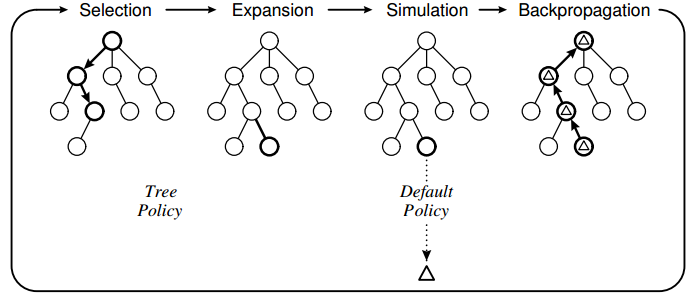
\includegraphics[width=\linewidth]{fig/mcts}
\caption[\gls{mcts}]{Illustration of how \gls{mcts} algorithms function.}
\label{fig:mcts}
\end{figure}

The main things this method tries to achieve are to approximate the value of actions through random simulations and to use values efficiently for a best-first strategy. While the agent in TD algorithms tries to learn a long term value for each state, its purpose in \gls{mcts} is to estimate temporary state values to decide the play of the next move. In this respect, it is an algorithm competing with $\alpha\beta$-search for deciding the next move. In general, minimax is considered to be an unsuitable choice if no reliable heuristic exists. For large branch factors \gls{mcts}'s ideas are also superior to minimax, as it is easier to gain depth. However, it is argued that \gls{mcts} performs poorly in tactical situations where the smallest mistake may be decisive \cite{rama11}. These considerations lead to the insight that it may be hard for \gls{mcts} to improve chess play, especially in comparison with minimax. On the other hand, as we are trying to assume no additional domain specific knowledge, the simulation aspect of \gls{mcts} could help things out. It feels like more research into this topic needs to be conducted.

\subsection{AlphaGo}
Here, we discuss how a \gls{mcts} algorithm has been implemented in \textit{AlphaGo}, as it may gain more insight how it could be beneficial to self play in a \gls{rl} game environment \cite{alphago16}.
The phases are constructed in the following way (figure \ref{fig:alphago}):
\begin{enumerate}
\item \textbf{Selection}. Each edge contains statistics about the results obtained previously under the tree and roll-out policy. The stored values for an edge corresponding with the action $a$ from state $s$ are the action value $Q(s,a)$, the visit count (the number of iteration passing through that node) $N(s,a)$ and a prior probability $P(s,a)$ representing the policy learned with a policy network, see section \ref{sec:polnet}. The tree policy for the selection phase is then defined to be
\begin{equation}
a_t=\text{argmax}_{a}\left\{Q(s_t,a_t)+u(s_t,a_t)\right\}
\end{equation}
where $u(s_t,a_t)\propto\frac{P(s,a)}{1+N(s,a)}$, hence $u(s,a)$ encourages exploration.
\item \textbf{Expansion.} From the leaf node on, the default policy (a faster version of the previous described network) is applied. If the child of the leaf has been visited a sufficient number of times, it will be added to search tree.
\item \textbf{Simulation.} A \gls{mc} roll-out yields the final result $r$ of the game under the default policy. 
\item \textbf{Backpropagation.} The value that will be propagated back to through the edges of the tree is
\begin{equation}
V(s_L)=(1-\mu)\hat{V}(s_L)+\mu r
\end{equation}
where $\hat{V}(s_L)$ is the estimation by feeding the leaf node through the neural network. All edges through the path of the search tree are updated according to the following rule:
\begin{align}
N(s,a) & \leftarrow N(s,a)+1 \\
Q(s,a) & \leftarrow (1-\frac{1}{N(s,a)})Q(s,a)+\frac{1}{N(s,a)}V(s_L)
\label{eq:mcts_update}
\end{align}
\end{enumerate}
where equation \ref{eq:mcts_update} is a moving average over all encountered leaf values.

\begin{figure}
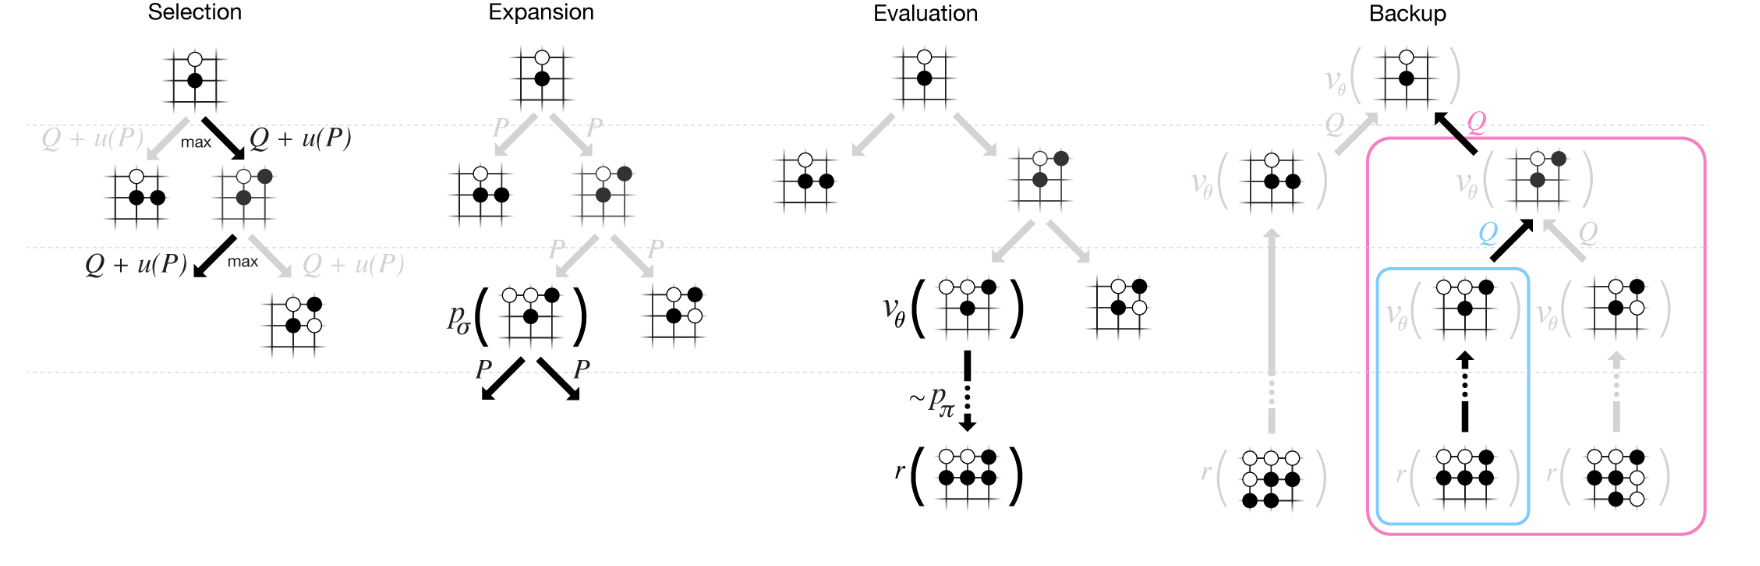
\includegraphics[width=\linewidth]{fig/alphago_mcts}
\caption[AlphaGo]{Illustration of the four phases of \gls{mcts} in \textit{AlphaGo}.}
\label{fig:alphago}
\end{figure}

\section{Policy Gradient Reinforcement Learning}
\label{sec:polnet}
Only approximating the value function has a big downside for deterministic games, namely that the smallest difference in value between two actions can cause a change in selection between moves \cite{sutton00}.
A common theme in learning to play games is to iterate between learning a value function and policy iteratively, as discussed in section \ref{subsec:iter}. For very large state spaces, which is the most common in game theory, this equals iterating between learning an approximation function $V_w(s)$ and a probability distribution $\pi_w(a|s)$. \\
Just as a deep neural network can be used to learn $V_w(s)$, the same is true for $\pi_w(a|s)$, where the difference in architecture between both is a softmax layer at the end instead of a single value learned with regression. Policy networks have proven their strengths in Go \cite{alphago16}.\\

Making policy networks a viable option for Go is the encoding of the actions, which is simply setting a stone at a certain square. Actions can thus easily be encoded with an output map. For chess, this encoding is much harder, as of al the legal actions possible in the game, at each state only a few are possible. An interesting research question is how policy networks can be incorporated into learning to play chess by finding decent encodings, especially for a CNN framework. A possible idea is the use of 2 output maps, one for the start position and one for the final position of a piece, hence encoding a uci move. This results in the encoding of $64^2$ actions, from which most of them are not legal, especially from a certain state where the average breadth is around 20. \\

Another potential idea is recent research into Atari games, where a new CNN architecture has been proposed to estimate the optimal advantage function, defined to be
\begin{equation}
A(s,a)=Q(s,a)-V(s)
\end{equation}
The dueling \gls{ddqn} learns $Q(s,a)$ by separately learning the advantage and the value in the same network. By estimating the advantage function, we can significantly reduce the variance on the policy, which is very state dependent, hence this network could be a better choice than separating with an individual policy network. The dueling \gls{ddqn} is the state of the art in playing Atari games \cite{dddqn15}.

\section{Monte Carlo Value Initialization}

All current \gls{rl} techniques in chess use some sort of expert knowledge for the time being. \textit{KnightCap} performed its training by playing humans and initializing its weights to piece value count, \textit{Giraffe} initialized its network weights in the same way and used grandmaster positions to start with. \textit{Meep} used handcrafted expert chess features. For the vision of this thesis, all these methods are forbidden, as they introduce some expert bias. At the same time, some initialization might be necessary to have a good point to start from and speed up training, as TD learning might take a very long time due to its nature to propagate back from the ending evaluation. The trick that made some of the previous chess engines quite successful was the initialization to a piece value count, as in this fashion, it is not necessary to branch out episodes up until the total end, the checkmate, which would be time consuming.\\

An own idea came to mind, trying to solve this issue. We will call the algorithm the \gls{mcvi}, as it heavily relies on \gls{mc} roll-outs. The idea is to set up random positions, and create a raw estimate of the value function based on the statistical results of the roll-out from that board position. As the statistics provide a value between 0 and 1, we transform it to be zero sum with the following equation:
\begin{equation}
V\leftarrow\frac{2w}{w+l}-1
\label{eq:v_mcvi}
\end{equation}
which provides as a number between -1 and 1, hence mimicking the optimal value function. As positions with less pieces are on average objectively closer to a terminal state with optimal play and easier to finish, we start off the algorithm with less pieces. After this, we can continue for more pieces and play until a certain confidence is reached over the positions by evaluating them through the network, as the network already learned how to handle these with raw evaluations for less pieces. This (obviously) saves out time, as we do not have to execute the simulations until a terminal state has reached, and stop preemptively. A rudimentary algorithm is depicted in \ref{al:mcvi}. \\
It is important to note how draws are not accounted in the calculations. We drop these simulations, as statistically speaking, by performing completely random actions without any peculiar policy, the relative difference between wins and losses would be minimized. The obtained values would not be a good indication about who got the better opportunities if play would be better.\\ 

\begin{algorithm}
\begin{algorithmic}
\REQUIRE $P,M,N$
\FOR{$i\leftarrow1$ to $P$}
	\STATE$\mathcal{D}\leftarrow\left\{\right\}$
	\FOR{$m\leftarrow1$ to $M$}
		\STATE{$B\leftarrow$ random position with $P$ pieces}
		\FOR{$n\leftarrow1$ to $N$}
			\STATE $w\leftarrow0$
			\STATE $l\leftarrow0$
			\STATE $r\leftarrow\text{MC-rollout}(B)$
			\COMMENT{until certain confidence from end result is reached}
			\IF{$r$ is a win}
				\STATE $w\leftarrow w+1$
			\ELSIF{$r$ is a loss}
				\STATE $l\leftarrow l+1$
			\ENDIF
		\ENDFOR
		\STATE $V\leftarrow\frac{2w}{w+l}-1$
		\STATE $\mathcal{D}\leftarrow\mathcal{D}\cup\left\{(B,V)\right\}$ 
	\ENDFOR
	\STATE fit $\mathcal{D}$ to network
\ENDFOR
\end{algorithmic}
\caption{Monte Carlo Value Initialization}
\label{al:mcvi}
\end{algorithm}

There are still some pitfalls that could ruin the joy:
\begin{itemize}
\item in some positions it is clear how play should continue, and how the side with the material advantage can win, but random play may benefit the other side. An example is illustrated in figure \ref{fig:mcvi1}.
\item Some positions are a draw, but random play may let the side that is the most probable to make a mistake do foolish actions, while the strategy maintaining the draw is straightforward (figure \ref{fig:mcvi2}).
\item To yield a good first rough estimate, many simulations may still be needed for every $P$.
\end{itemize}
We may hope, that these strange positions are exceptions, and that the law of big numbers may weaken their influence.

\begin{figure}
\centering
    \begin{subfigure}[t]{0.45\textwidth}
        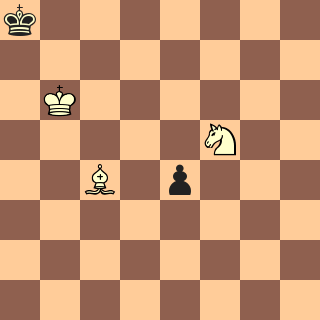
\includegraphics[scale=0.5]{fig/diagram_mcvi}
        \caption{white is on the winning hand here, but black is more probable to win with random moves. The probability is sufficiently high that the black pawn will succeed at promoting to a queen, while setting the mating net is not straightforward to accomplice with the white pieces.}
        \label{fig:mcvi1}
    \end{subfigure}
    \qquad
    ~ %add desired spacing between images, e. g. ~, \quad, \qquad, \hfill etc. 
      %(or a blank line to force the subfigure onto a new line)
    \begin{subfigure}[t]{0.45\textwidth}
        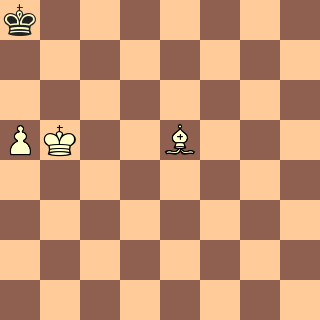
\includegraphics[scale=0.5]{fig/diagram_mcvi2}
        \caption{To hold a draw, black can just move back and forward from a8 and b7. The problem is that black will make mistakes by playing randomly, and white will achieve an evaluation of 1 with equation \ref{eq:v_mcvi}.}
        \label{fig:mcvi2}
    \end{subfigure}
    ~ %add desired spacing between images, e. g. ~, \quad, \qquad, \hfill etc. 
    %(or a blank line to force the subfigure onto a new line)
    \caption{Two examples leading to bad $MC$ evaluations.}
\end{figure}

To conclude this section, let us make a final remark about our vision in this document. We assume the agent should know nothing more than the rules at the beginning of the game. If we change this vision, to creating a chess engine that learns to play chess by only accepting objective facts, we could modify our \gls{mcvi} algorithm in such a way to create a satisfying initialization with more certainty, by simply looking at the evaluation of tablebases (see section \ref{subsec:tablebases}). If the position drawn from a MC roll-out seems to be in the tablebase, a correct result can be returned instantly, heavily improving the algorithm.